\chapter{Introduzione}
\section{Premessa}
Nonostante il grande successo della trasformazione digitale, molti ambiti delle nostre interazioni sono rimasti datati e non si sono adattati al digitale; un esempio su tutti è quello del settore legale. Detto ciò, è importante anche notare che la digitalizzazione presenta anche lati oscuri \cite{La_quarta_rivoluzione_industriale}: i nostri dati sono controllati da organizzazioni il cui obiettivo principale è il profitto, gli hacker tentano continuamente di sottrarre informazioni personali e gli Stati monitorano le attività dei cittadini per mantenere l’ordine e il controllo.

\section{Come nasce la Blockchain}
\begin{wrapfigure}{r}{0.25\textwidth} %this figure will be at the right
    \centering
    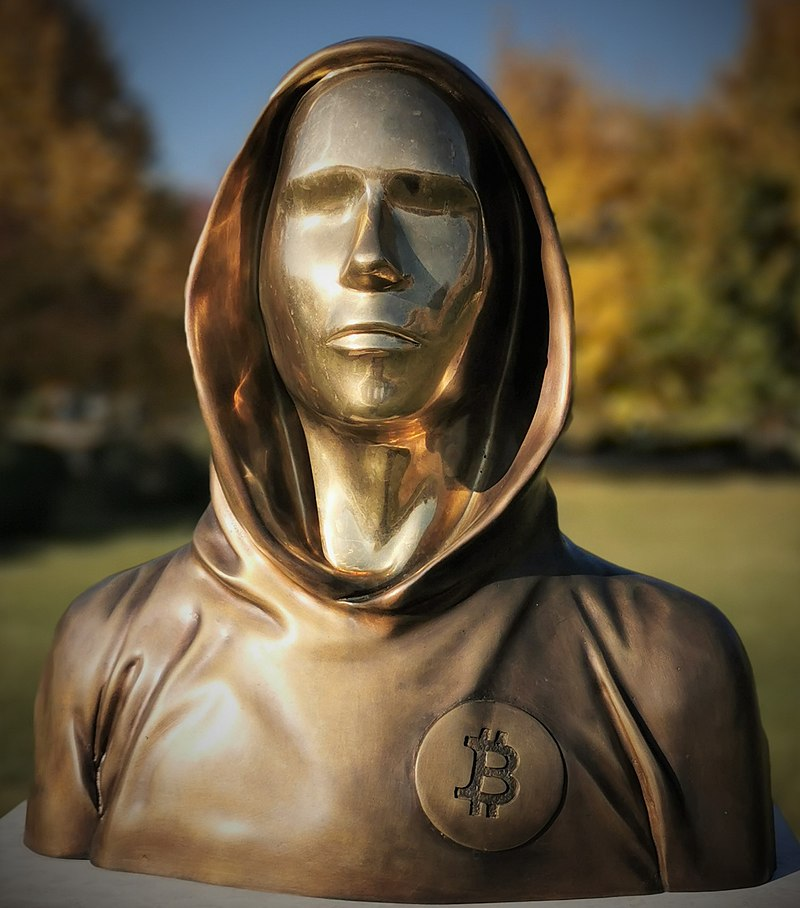
\includegraphics[width=0.25\textwidth]{Immagini/Satoshi_Nakamoto.jpg}
    \caption{Statua raffigurante Satoshi Nakamoto}
\end{wrapfigure}
Tutto ha origine nel 2008, con la pubblicazione online dell’articolo “Bitcoin: A Peer-to-Peer Electronic Cash System” da parte di Satoshi Nakamoto, pseudonimo che potrebbe celare un individuo o un gruppo di persone. L’obiettivo del documento era quello di creare un sistema puramente peer-to-peer per il trasferimento di valore tra le parti, eliminando la necessità di intermediari come banche o istituti finanziari.
Il concetto chiave della blockchain è la possibilità di creare una generazione di piattaforme decentralizzate e disintermediate, nelle quali la fiducia tra le parti non è garantita da un’organizzazione centrale, ma dalla piattaforma stessa, attraverso un meccanismo algoritmico: essa si riferisce, in senso più ampio, all’insieme di tecnologie che rendono possibile la decentralizzazione, basandosi sul modello peer-to-peer.
In sostanza consente di immaginare un mondo organizzato in modo completamente diverso.
